\chapter{EPANET framework}
\label{epanet_framework_appendix}

\emph{This chapter gives an insight into the simulation model of the Randers WSS in EPANET. In order to understand better how the simulation works, the modelling of the different pumping stations, waterworks, and the consumption patterns are explained in detail. In the end, an attempt is made to split the network into different subsystems and make necessary modifications such that data is sufficiently reduced and therefore easily extractable for system identification purposes.}

% \emph{This chapter gives a general introduction about the need for model simplification in WSSs. Different approaches and methods are discussed in a state of art manner, including the development and methodologies employed in this field. Lastly, an attempt is made to simplify the Randers WSS, using one of the techniques which are being introduced in this chapter. }



\section{Model calibration and validation}
\label{model_calibration_and_validation}

The simulation data has been validated by using pressure measurements on different fire hydrants in the network for several times corresponding to different years. When the model was made, the data was not completely up to date, as these pressure measurements were carried out in years before the EPANET modelling. The major uncertainty about this data is in the arrangement of the pipe network and the pumping stations, since it has been changed over the years and old facilities have been replaced. Although the data on which the model relies is uncertain and there might be variations in pressure, the validation of the model has been carried out according to these highly uncertain pressure measurements. 

\subsection{Pipe roughness}
\label{pipe_roughness}

In the model, all pipes are associated with tags, indicating dimensions, material and year information. With this information it is possible to estimate an average resistance, i.e. roughness of the pipes. 
During the validation process of the pipe resistances, it was chosen to consider an average roughness value, taking into account that the roughness should not be lower than a roughness of new pipes and at the same time, should not exceed a certain upper bound. Roughnesses were upscaled at places where the pressure was too high while downscaled where the pressure was certainly too low. Correct pressure data, however is an essential information for a more detailed and precise calibration, therefore high deviations up to 5 meter heads are present in the system. \figref{fig:pressure_mistakes} shows the pressure deviation in the system compared to the data on which the system was calibrated. 

%Fire hydrants measurements
\begin{figure}[H]
\centering
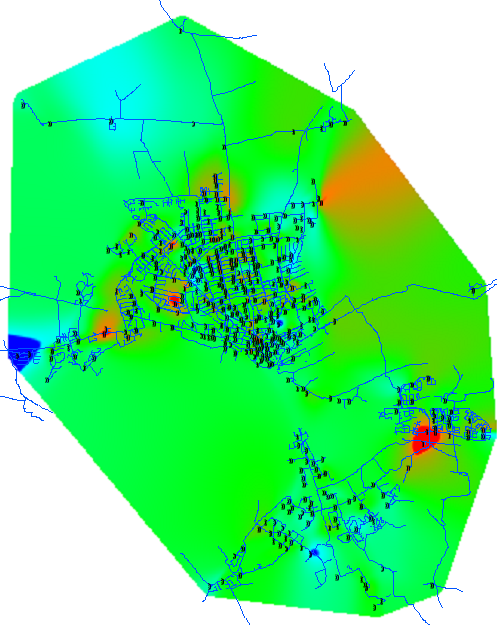
\includegraphics[width=0.55\textwidth]{report/pictures/fire_hydrants}
%\begin{tikzpicture}[scale=0.6,transform shape]

\begin{scope} [rotate around={0:(12,5.5)}, shift={(0.8,0)}]
\draw[thick,transform shape] (12,5.5) circle (0.5);
\draw[thick,transform shape] (12.5,5.5) -- (12,6);
\draw[thick,transform shape] (12.5,5.5) node (v1) {} -- (12,5);
\end{scope}

%man-valve
\begin{scope} [rotate ={-90}]
\node(n1) at (-5.25,16) {};
\draw[thick,transform shape](n1.center) -- ($(n1)-(0.5,0)$) --
($(n1)-(0,1)$) -- ($(n1)-(0.5,1)$) --  (n1.center);

\end{scope}

\draw [thick](15,5.5) -- (13.3,5.5);
\node at (15.5,6.2) {\large PRV};
\draw [thick](16,5.5) -- (17.5,5.5);
\draw [fill=cyan] [thick](9.1,5.7) -- (9.1,5.1) -- (10.9,5.1) -- (10.9,5.7);
\draw  [thick](9.1,6.1) -- (9.1,5.1) -- (10.9,5.1) -- (10.9,6.1);
\draw [thick](12.3,5.5) -- (10.9,5.5);
\end{tikzpicture} 
\caption{Difference calculation between observed and calculated pressures on fire hydrants\cite{verdo_doc}.}
\label{fig:pressure_mistakes}
\end{figure}

\vspace{-3mm}

\subsection{Grid balance and supply zones}
\label{grid_balance_supply_zones}

With the simulation model in EPANET there is a possibility to illustrate which pumping stations supply the different areas in the network. Simulations can be carried out for instance on supply areas in certain zones where more than one pumping station contributes to the consumption. The two zones, considered in this report are the HZ and LZ, in which the former is supplied by OMV and TBP and the latter is supplied by HBP and HSP where the tanks are placed on high elevation level. Consequently, as mentioned in \secref{waterworks_and_pumping_stations}, OMV and TBP are the waterworks and pumping stations which are responsible for filling the tanks in the HZ in HBP and HSP, respectively. 
Using the water quality properties of EPANET, a contamination was introduced first in OMV pumping station and then TBP. By introducing a contamination into the system, it can be tracked which parts of the network gets contaminated. \figref{fig:HSP_HBP_EPA} shows an example for this, illustrating the distribution between the two pumping stations, OMV and TBP. 


\begin{figure}[H]
\centering
\begin{subfigure}{.49\textwidth}
\centering
  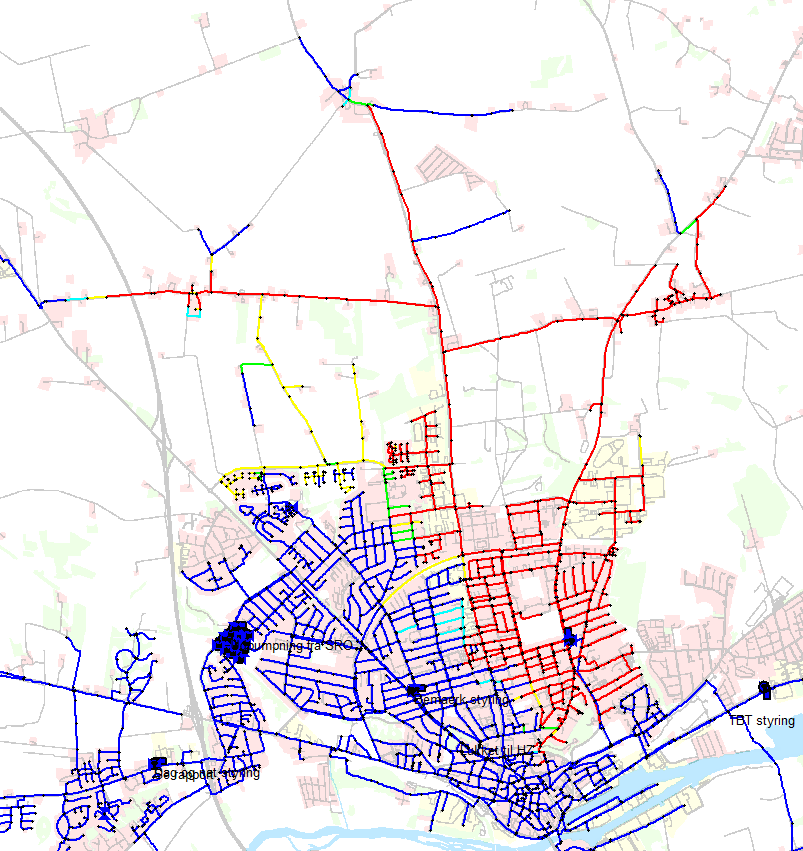
\includegraphics[width=0.75\textwidth]{report/pictures/HBP_HSP_distribution}
  \caption{HSP supply area, marked with red}
  \label{fig:HSP_HBP_EPA1}
\end{subfigure}
\begin{subfigure}{.49\textwidth}
\centering
  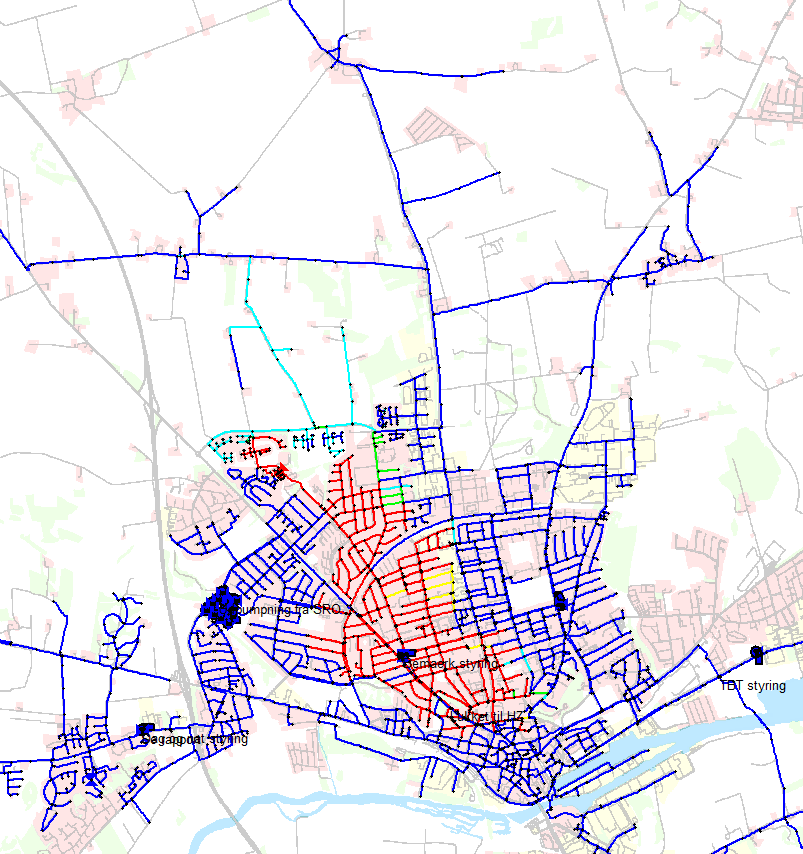
\includegraphics[width=0.75\textwidth]{report/pictures/HBP_HSP_distribution1}
  \caption{HBP supply area, marked with red}
  \label{fig:HSP_HBP_EPA2}
\end{subfigure}
\caption{Supply area by HSP(on the left) and supply area by HBP(on the right)\cite{verdo_doc}.}
\label{fig:HSP_HBP_EPA}
\end{figure}

\vspace{-3mm}

The red areas in \figref{fig:HSP_HBP_EPA} indicate 80-100 percent of drinking water originating from one or the other pumping station. However, the other colours(primarily yellow and green) indicate that there is a mix of water from both stations. The result in the grid is according to the control goals, as one pumping station supplies half of the region and an other the other one. This is achieved by controlling the flow in HBP and the pressure in HSP. 